% Build with XeLaTeX from this directory. The vector figure and its Python
% regeneration script are in figures/. The original October note is separate.
\documentclass[11pt]{article}
\usepackage[a4paper,top=17mm,bottom=20mm,left=18mm,right=18mm,footskip=10mm]{geometry}
\usepackage{fontspec,graphicx,xcolor,booktabs,tabularx,fancyhdr,hyperref}
\IfFontExistsTF{Georgia}{\setmainfont{Georgia}}{\setmainfont{TeX Gyre Pagella}}
\IfFontExistsTF{Arial}{\setsansfont{Arial}}{\setsansfont{TeX Gyre Heros}}
\IfFontExistsTF{Consolas}{\setmonofont{Consolas}}{\setmonofont{Latin Modern Mono}}
\definecolor{ink}{HTML}{203442}
\definecolor{teal}{HTML}{11645F}
\definecolor{muted}{HTML}{56686F}
\definecolor{hair}{HTML}{AEBFBE}
\hypersetup{colorlinks=true,urlcolor=teal,linkcolor=teal,pdfauthor={Zhijing Wu},
  pdftitle={When a world model changes the planner's first action},pdflang={en-US},
  pdfsubject={State ownership in executable world-model search}}
\pagestyle{fancy}\fancyhf{}\renewcommand{\headrulewidth}{0pt}
\renewcommand{\footrulewidth}{0.35pt}
\renewcommand{\footrule}{\hbox to\headwidth{\color{hair}\leaders\hrule height\footrulewidth\hfill}}
\fancyfoot[L]{\sffamily\fontsize{9}{11}\selectfont\color{muted}Zhijing Wu \enspace/\enspace Sichuan University \enspace/\enspace November 2026}
\fancyfoot[R]{\sffamily\fontsize{9}{11}\selectfont\color{muted}\thepage\ / 2}
\setlength{\parindent}{0pt}\setlength{\parskip}{5pt}
\setlength{\emergencystretch}{2em}\raggedbottom
\newcommand{\eyebrow}[1]{{\sffamily\bfseries\color{teal}\fontsize{9.5}{12}\selectfont #1}\par}
\newcommand{\heading}[1]{\vspace{4pt}{\sffamily\bfseries\fontsize{14}{17}\selectfont #1\par}\vspace{-1pt}}
\newcommand{\titleline}[1]{{\sffamily\bfseries\fontsize{25}{29}\selectfont #1\par}}
\newcommand{\src}[2]{\mbox{\href{#1}{\sffamily\fontsize{9}{11}\selectfont #2}}}
\newcommand{\repo}{https://github.com/ZhijingWu/world-model-planning-reliability/blob/}
\newcommand{\vone}{\repo 11ddff4d1a3a7af5da2728c0b5e368b8573c41ee/studies/sciworld-fixed-work-v1/}
\newcommand{\vtwo}{\repo 8c6bfc9dc92f3e0e53be7def3b867036cb1b8e2a/studies/sciworld-prospective-v1/}
\newcommand{\runtime}{\repo 4ba67940378b959a07e63426cf4d3d3bdaf93c86/}
\newcommand{\original}{\repo 3c9022030323bd22e05b3f5276531eaa542cb1eb/}
\newcommand{\rawmodel}{\original third_party/PatchWorld/examples/generated_world_models/sciworld_benchmark_world_model.py}
\begin{document}
\color{ink}\fontsize{11}{15}\selectfont
\eyebrow{WORLD MODEL PLANNING RELIABILITY \enspace/\enspace RESEARCH NOTE}
\titleline{When a world model changes\\the planner's first action}
A search evaluates alternatives by returning to a shared parent state. What happens if
one simulated action returns the expected successor but also changes that parent?
In a prospective test on the released SciWorld program, this difference in how branches
were executed changed the selected first action on \textbf{7 of 64} sampled states.
\src{\vtwo public/analysis.json}{Prospective results}

\heading{Follow one write through a search}
PatchWorld generates executable models from trajectories. Its released SciWorld
model starts a transition with a shallow copy of the belief dictionary. A write to
the nested \texttt{object\_states} mapping can therefore reach the caller. In the
case below, the writer returned the same successor as Full Copy, but the next
sibling read a different input and gained one goal-field match.
\src{https://arxiv.org/abs/2605.30880v4}{Bai et al., 2026}\enspace
\src{\rawmodel}{Model source}\enspace\src{\vone public/report.md}{Case evidence}

\vspace{2pt}
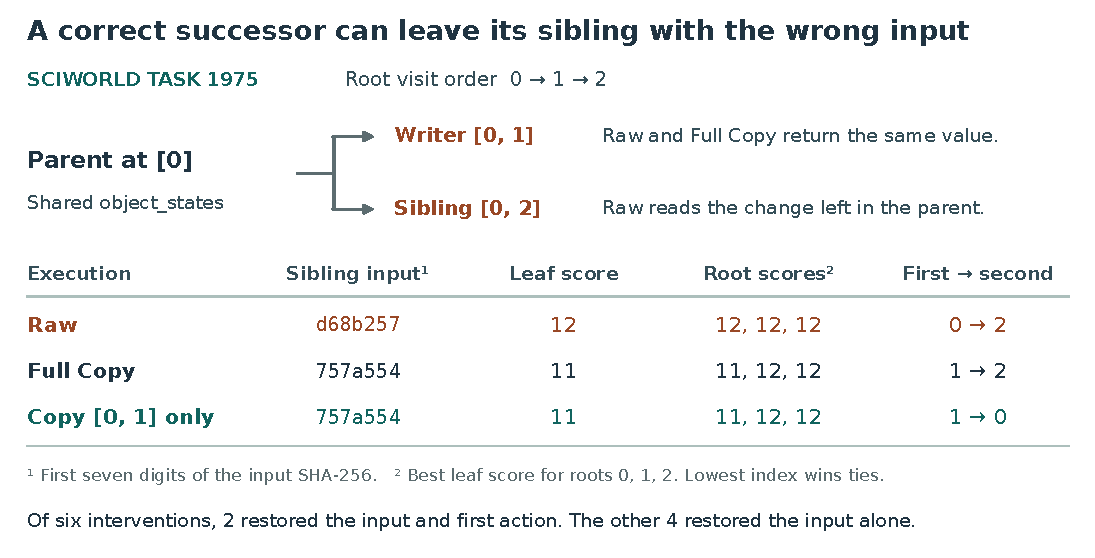
\includegraphics[width=\linewidth]{figures/task-1975.pdf}\par
{\sffamily\fontsize{9.4}{12}\selectfont\color{muted}
\textbf{Figure 1.} Brackets give candidate indices along an edge. Isolating the writer
restored the reference first action in this order. The chosen second action still differed.
\src{\vone public/results.json}{Edge records}\par}

The original study examined nine states selected for a historical replay failure and
two comparison states. Task 1975 alone changed the first action across that bank.
The selection procedure left the frequency of this mechanism on new states open.
\src{\vone public/manifest.json}{Original selection}\enspace\src{\vone public/verification.json}{Verification}

\heading{An independent reference and an isolation runtime}
\textbf{Raw} calls the original model on the live parent. \textbf{Full Copy} calls the
same model on a fresh deep copy at every edge. This defines a reference for the
program's own dynamics. OpenSpiel's \texttt{Child} method likewise clones the
parent before applying an action in a game.
\src{https://arxiv.org/abs/1908.09453}{Lanctot et al., 2019}\enspace
\src{https://github.com/google-deepmind/open_spiel/blob/82b5aac85c577b6911f9a912544e2a589dacc2f1/open_spiel/spiel.h\#L562-L570}{OpenSpiel interface}

\textbf{WCTR}, short for Witness-Compiled Transactional Rollouts,
uses observed write paths to copy selected containers and aliases, records unexpected
supported writes, and restores the parent. Uncertain inputs or source forms can trigger
Full Copy. The contract covers trusted, deterministic, state-confined models with
plain-data results. \src{\runtime docs/SUPPORTED_STATE.md}{Released contract}

\newpage
\fontsize{11.5}{16.4}\selectfont
\eyebrow{PROSPECTIVE STUDY \enspace/\enspace SCIWORLD}
\titleline{How often did the first action change?}
The protocol excluded the original trajectories and overlapping source items, then
sampled one preassigned state per item without replacement. Candidate commands came
from the whole logged trajectory. A command could first appear later and be unavailable
at the root in an online environment. A model walk generated each synthetic goal.
All arms evaluated three roots and three children per root, using 12 transitions
for each of six visit orders. The best leaf's count of matching goal fields scored
its root. The primary rule broke ties by lowest candidate index.
\src{\vtwo protocol.md}{Protocol}\enspace\src{\vtwo public/manifest.json}{Frozen sample}

\heading{Seven of 64 states changed the selected first action}
A state counted once if any visit order changed the decision. The estimate was
\textbf{10.94\%} with an exact 95\% finite-frame interval of \textbf{5.63--19.48\%}
for the 231 eligible representatives. The six orders are repeated measurements of
each state. All trials use one generated program. \src{\vtwo public/analysis.json}{Estimates and counts}

{\sffamily\fontsize{10.5}{14}\selectfont
\renewcommand{\arraystretch}{1.17}
\begin{tabularx}{\linewidth}{@{}Xrr@{}}
\toprule
\textbf{Raw versus Full Copy} & \textbf{States of 64} & \textbf{Orders of 384}\\
\midrule
A later input differed & 15 & 90\\
Set of best root actions differed & 8 & 46\\
First action differed under the primary tie rule & 7 & 28\\
First action differed under the highest-index tie rule & 3 & 10\\
\bottomrule
\end{tabularx}\par}

In 62 paired orders, at least one score changed while the selected first action
stayed the same. The frozen candidate order mattered when the best actions tied.
\src{\vtwo public/analysis.json}{Order outcomes}

\textbf{Interventions.} On the 28 differing orders, isolating the earliest traced
writer restored both the affected sibling input and the reference first action in
10 orders across six states. In the other 18, the input recovered and the first
action still differed. Every affected state had at least one unresolved order.
Full Copy had a tied maximum in all 384 orders. Raw produced a strict winner in
12 orders. Switches between two strict winners therefore remain untested.
\src{\vtwo public/analysis.json}{Sensitivity and rescues}

\textbf{Replay and runtime.} Raw claimed an exact goal that failed independent
replay in 24 of 384 orders. Full Copy and WCTR had zero false goals. WCTR preserved
parents and matched the reference on all 4,608 search calls. It executed a whole-state
copy on every call. These trials therefore give no timing evidence for selective
forks. \src{\vtwo public/verification.json}{Trace verification}\enspace
\src{\vtwo public/analysis.json}{Replay counts}

\heading{Limits and the next test}
In earlier time-limited program search, WCTR completion relative to Full Copy rose
by 17.5 percentage points on WebShop and fell by 9.2 on Wordle. Native completion
tied across four protected methods at 6/12 WebShop goals and 43/100 Wordle seeds.
The 33,692 native WCTR checks belong to that historical runtime.
A pre-release 64-row diagnostic found a higher first-append cost and a lower
calibrated-append cost than Full Copy on the same fixture.
\src{\original CLAIMS_AND_LIMITATIONS.md}{Historical evidence}\enspace
\src{\runtime diagnostics/ast-gate/README.md}{Cost diagnostic}

Value-aware model estimation motivates measuring errors through their decision
consequences. On separate development data, select a score that yields positive
reference winner margins. Freeze it, then test whether contamination can reverse
those margins on new models. Native interaction would test whether different
actions change task success. \src{https://proceedings.mlr.press/v54/farahmand17a.html}{Farahmand et al., 2017}
\end{document}
